
\section{Руководство пользователя}

Для использования системы необходимо:
\begin{itemize}
\item{
 Чтобы она была установлена и настроена в соответствии с Руководством администратора.
}
\item{
 Веб-сервер доступен по сети из рабочей станции пользователя.
}
\item{
 На рабочей станции пользователя установлен один из веб-браузеров: 
Internet Explorer (версия >= 7), Google Chrome (версия >= 15.0), Firefox (версия >= 3.0).
}
\end{itemize}


\subsection*{Начало работы}

В начале работы пользователь вводит в адресную строку браузера URL-адрес веб-сервера.
В случае, если сессия не была инициализирована, будет открыта страница входа.

\begin{figure}[!ht]
\begin{center}
\hspace*{-1cm} 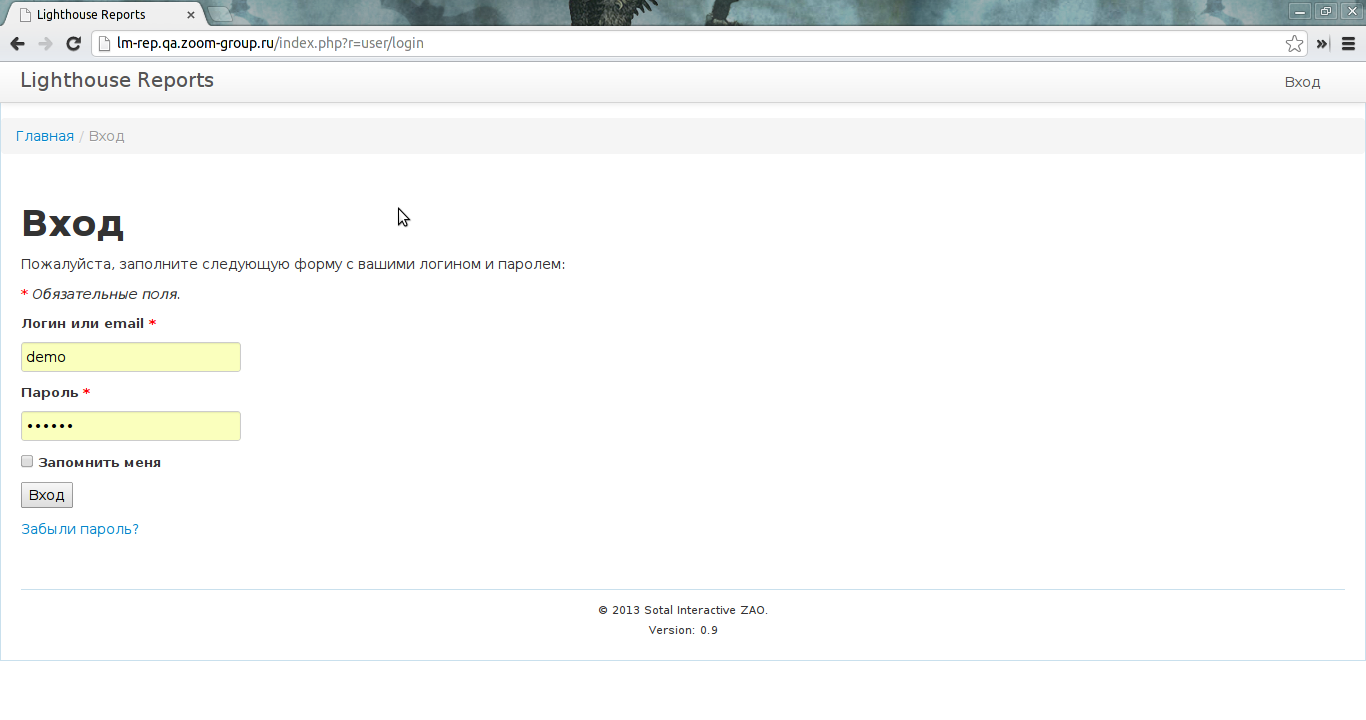
\includegraphics[scale=0.35, trim=0mm 0mm 0mm 10mm, clip]{../resources/screens/login.png}
\end{center}
\end{figure}

\begin{figure}[!ht]
\begin{center}
\hspace*{-1cm} 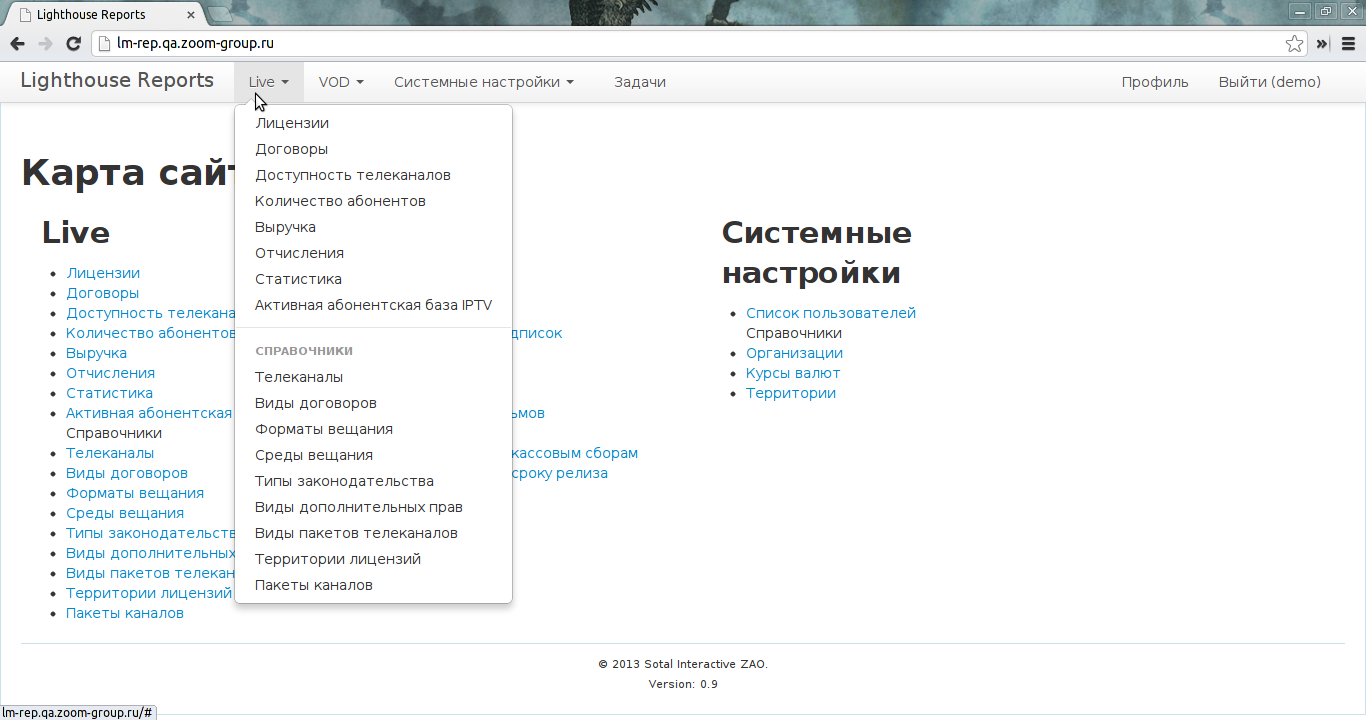
\includegraphics[scale=0.28, trim=0mm 0mm 0mm 10mm, clip]{../resources/screens/map.png}
\end{center}
\end{figure}

\vspace*{-1cm} 

После ввода правильных аутентификационных реквизитов, открывается Карта сайта, на котором
выведены все доступные пользователю разделы системы. Кроме карты сайта, доступные разделы
также расположены в Главном меню.

Приложение состоит из трех разделов: Live, VOD и Системные настройки.

\subsection*{Работа с данными}

Большая часть ссылок из подразделов предоставляют интерфейс для поиска/редактирования данных
определенного вида (примеры на рисунках).

\begin{figure}[!ht]
\begin{center}
\hspace*{-1cm} 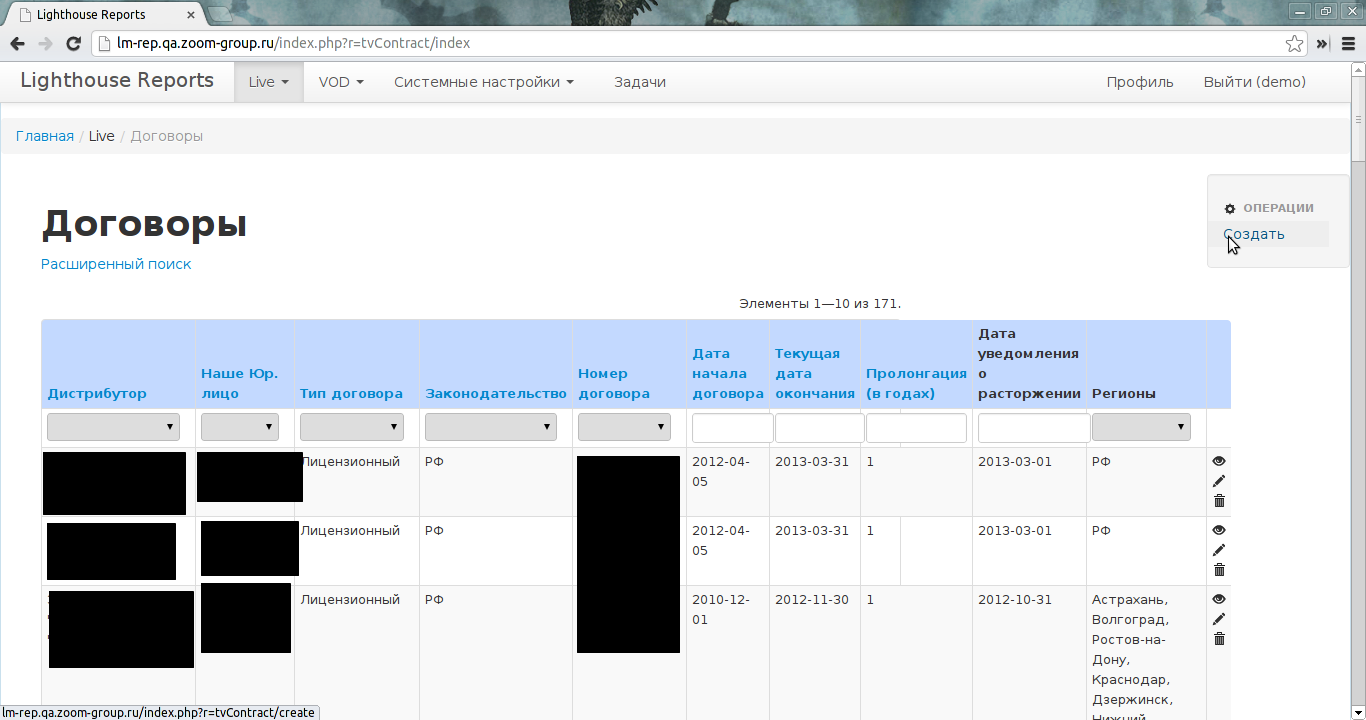
\includegraphics[scale=0.35, trim=0mm 0mm 0mm 10mm, clip]{../resources/screens/contracts.png}
\caption{Главная страница подраздела Live -> Договоры}
\end{center}
\end{figure}

\begin{figure}[!ht]
\begin{center}
\hspace*{-1cm} 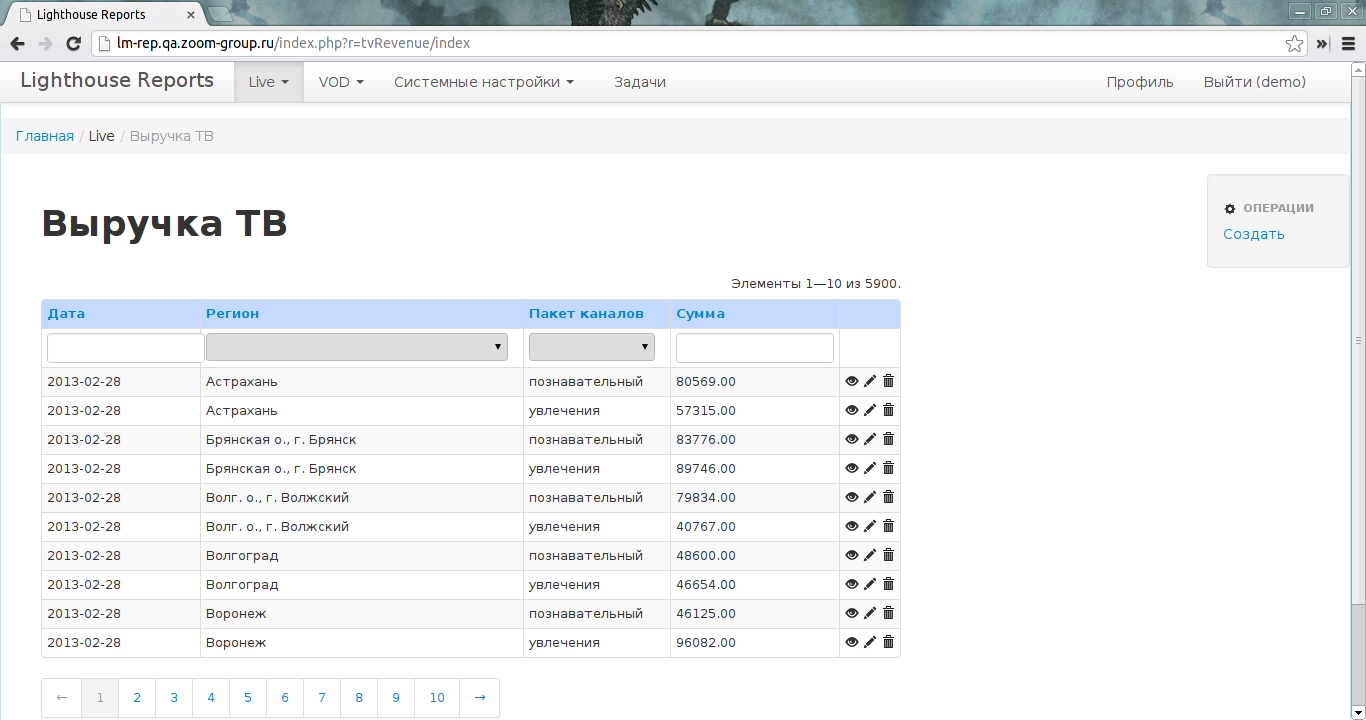
\includegraphics[scale=0.35, trim=0mm 0mm 0mm 10mm, clip]{../resources/screens/tv_revenue.png}
\caption{Главная страница подраздела Live -> Выручка ТВ}
\end{center}
\end{figure}

\begin{figure}[!ht]
\begin{center}
\hspace*{-1cm} 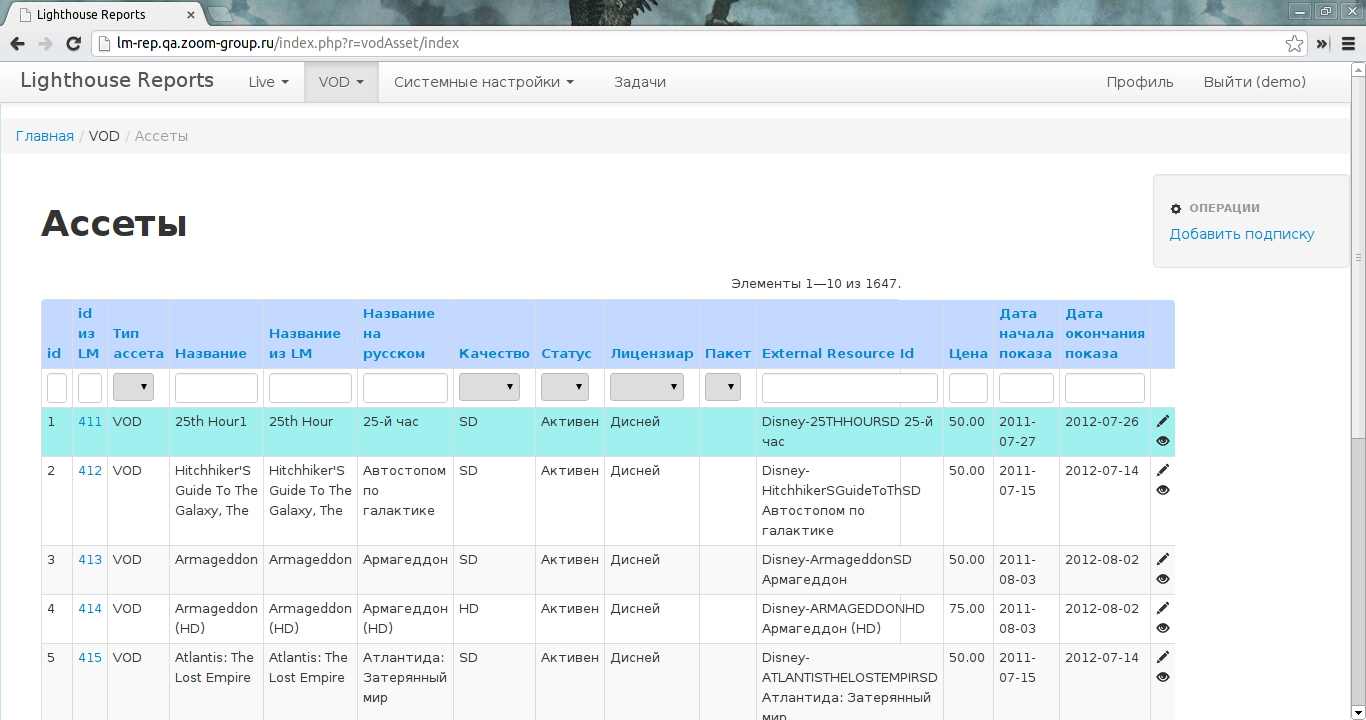
\includegraphics[scale=0.35, trim=0mm 0mm 0mm 10mm, clip]{../resources/screens/assets.png}
\caption{Главная страница подраздела VOD -> Ассеты}
\end{center}
\end{figure}

Находясь на главной странице такого интерфейса, пользователю доступен список объектов в виде таблицы.

Для фильтрации по значению нужно ввести необходимо ввести ключевое слово над соответствующим столбцом,
после чего произойдет обновление содержимого.

Для указания поля сортировки необходимо кликнуть по тексту заголовка соответсвующего столбца. 
Повторные нажатия изменят порядок сортировки или вернут сортировку по умолчанию.

В большинстве подобных интерфейсов присутствуют дополнительные операции, такие как например добавление объекта
(на рисунках в правом верхнем углу).

Для просмотра отдельного объекта нужно кликнуть по иконке с глазом в соответствующей строке.

Для редактирования объекта необходимо нажать на иконку с изображением карандаша, после этого браузер пользователя
перенаправляется на страницу редактирования.

\begin{figure}[!ht]
\begin{center}
\hspace*{-1cm} 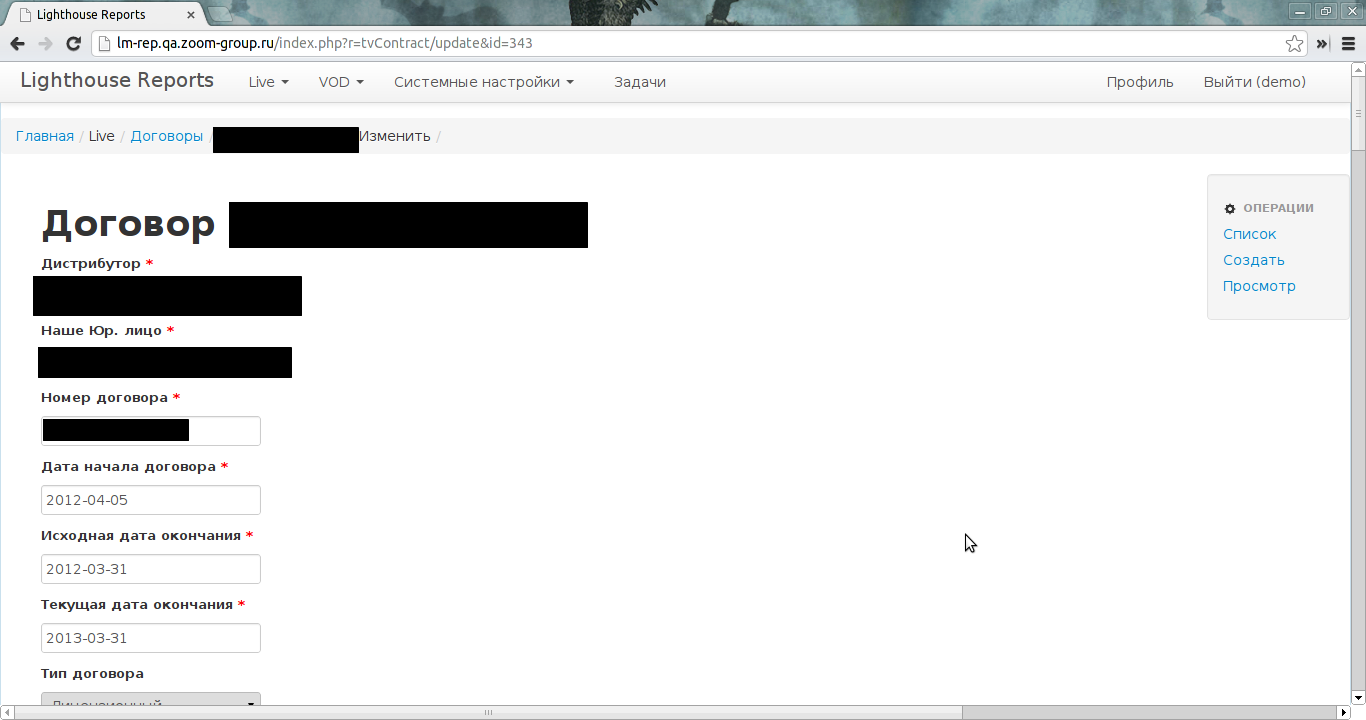
\includegraphics[scale=0.35, trim=0mm 0mm 120mm 10mm, clip]{../resources/screens/contract_edit.png}
\caption{Страница редактирования подраздела Live -> Договоры}
\end{center}
\end{figure}

\begin{figure}[!ht]
\begin{center}
\hspace*{-1cm} 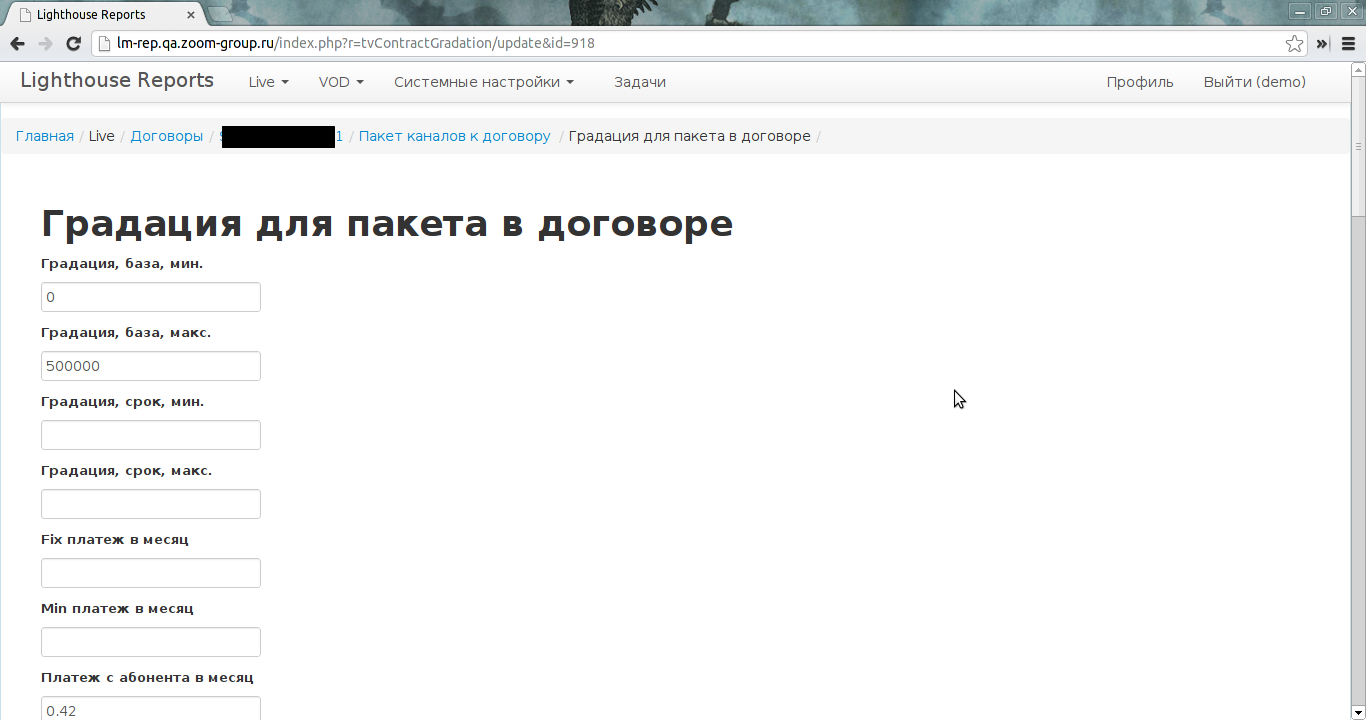
\includegraphics[scale=0.35, trim=0mm 0mm 120mm 10mm, clip]{../resources/screens/contract_gradation.png}
\caption{Страница редактирования градации по договору Live}
\end{center}
\end{figure}

На страницах с формами для редактирования/добавления объектов пользователь может заполнить
необходимые поля и сохранить объект, нажав кнопку "Сохранить" в нижней части страницы.

\begin{figure}[!ht]
\begin{center}
\hspace*{-1cm} 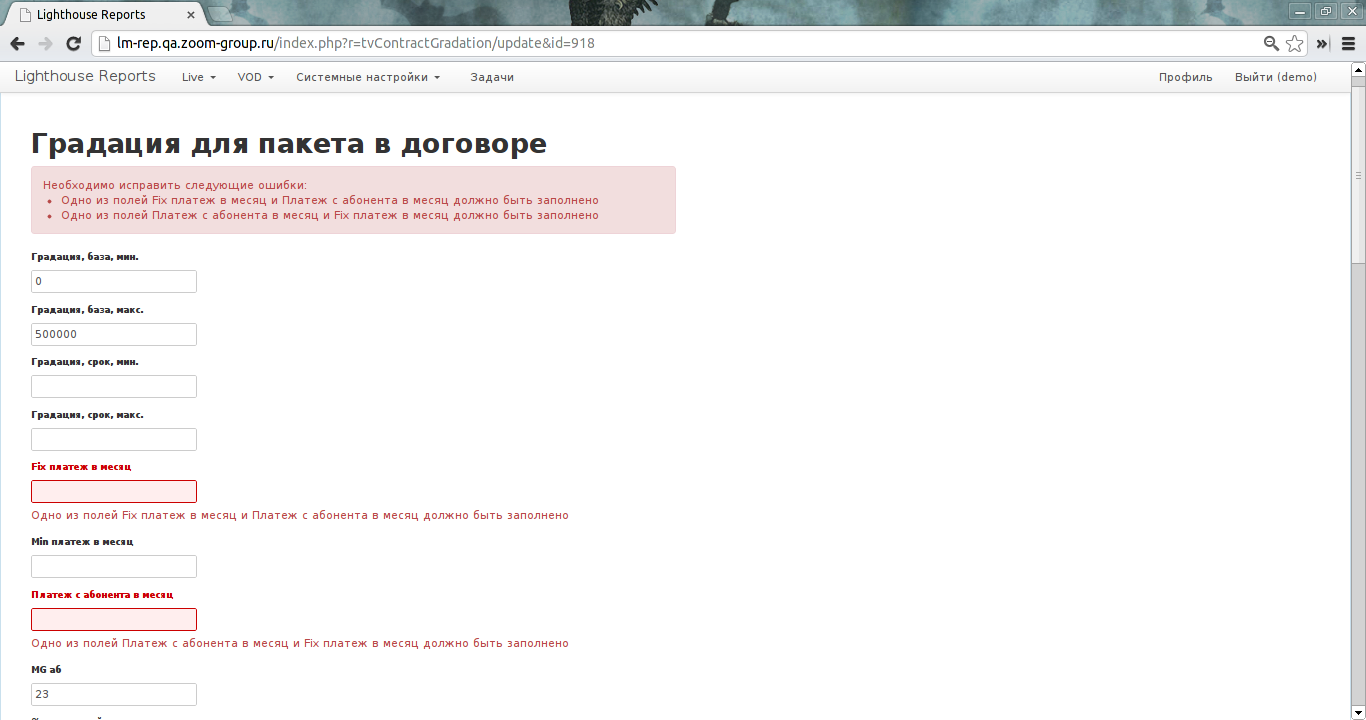
\includegraphics[scale=0.35, trim=0mm 0mm 120mm 10mm, clip]{../resources/screens/contract_gradation_error.png}
\caption{Страница редактирования градации по договору Live. Ошибка}
\end{center}
\end{figure}

В случае если данные формы были заполнены некорректно, объекты не сохраняются,
пользователю выводится уведомление в верхней части страницы. 
Кроме того поля с ошибочными значениями подсвечиваются красным цветом.

\subsection*{Задачи}

\begin{figure}[!ht]
\begin{center}
\hspace*{-1cm} 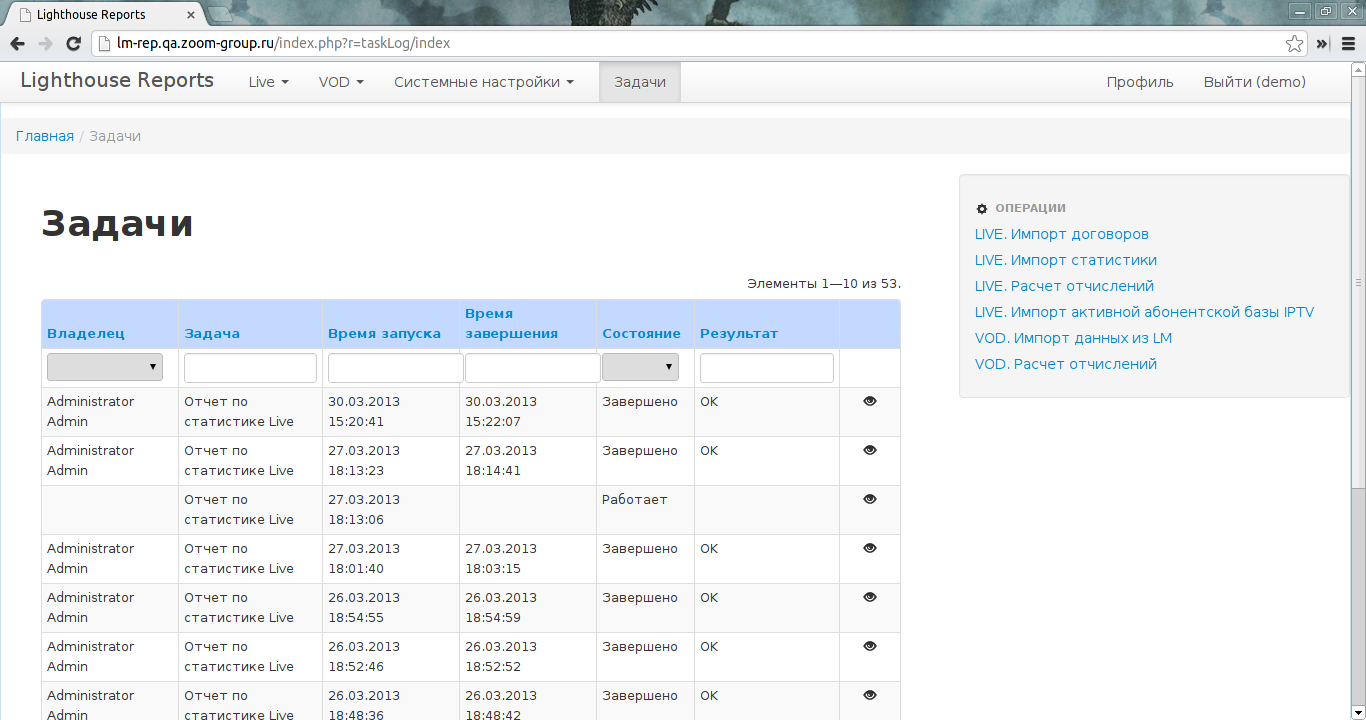
\includegraphics[scale=0.35, trim=0mm 0mm 0mm 10mm, clip]{../resources/screens/tasks.png}
\caption{Раздел задачи}
\end{center}
\end{figure}

В разделе "Задачи" пользователь может отслеживать статус запущенных им фоновых задач
и инициировать запуск новых.

Для просмотра результата завершенной задачи нужно кликнуть по пиктограмме с изображением глаза,
в случае, если результатом работы задачи был файл, он доступен для скачивания.

Для запуска доступны следующие задачи:
\begin{itemize}
\item{
  Импорт договоров по Live из файла в формате Microsoft Excel
}
\item{
  Импорт статистических данных по Live из файла в формате XML
}
\item{
  Расчет отчислений по Live
}
\item{
  Импорт активной абонентской базы из файла в формате Microsoft Excel
}
\item{
  Импорт данных для VOD 
}
\item{
  Расчет отчислений по VOD
}
\end{itemize}

\begin{figure}[!ht]
\begin{center}
\hspace*{-1cm} 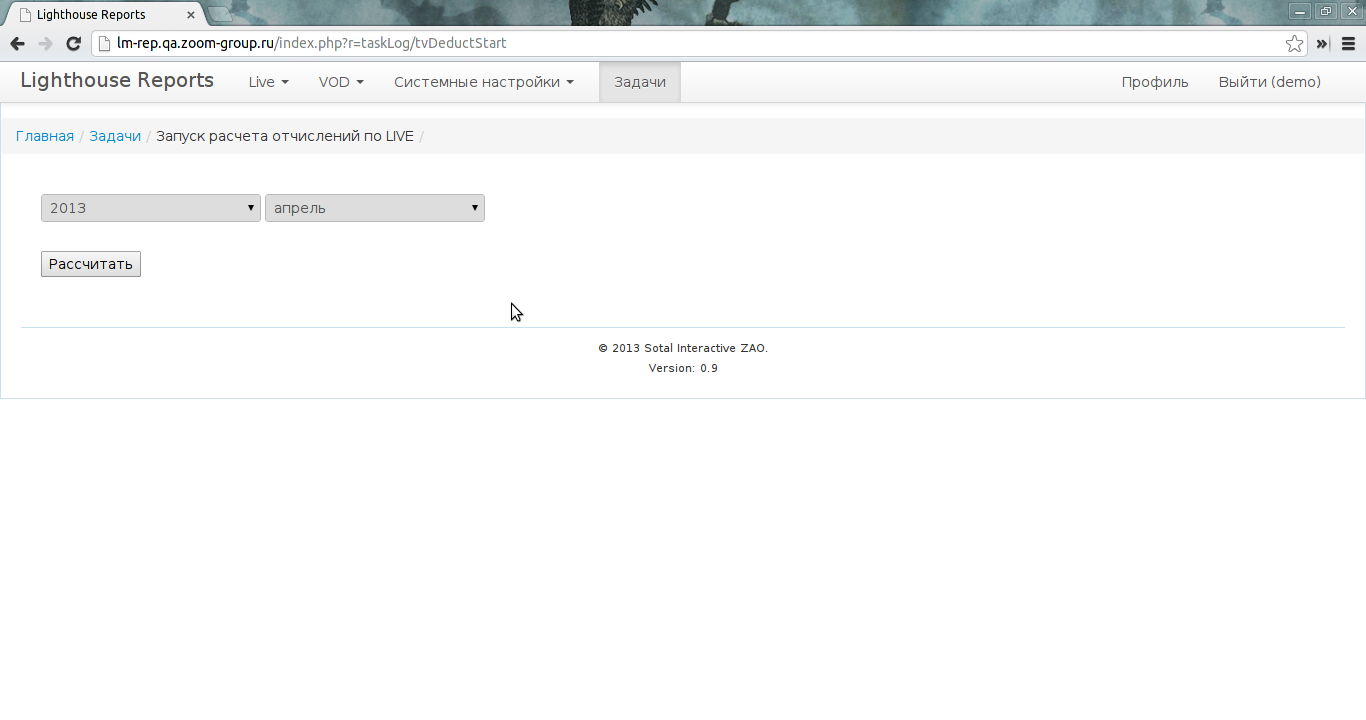
\includegraphics[scale=0.35, trim=0mm 70mm 250mm 10mm, clip]{../resources/screens/deduct_start.png}
\caption{Интерфейс запуска для расчета отчислений по Live}
\end{center}
\end{figure}

\subsection*{Генерация отчетов}
